Translation, as we have seen in Section \ref{sc:fgt}, is forming the local expansion at a target box by combining the plane-wave expansions of all source boxes in its interaction list.  The cost of the direct scheme (\ref{e:w2l}) is $\bigO(K^3 p^3 |B|)$. For uniform distributions, the {\em sweeping algorithm} introduced in \cite{greengard98} and extended to multi-dimensions in \cite{fggt} brings down the complexity to $\bigO(9p^3 |B|)$. 

For nonuniform distributions, we do not form plane-wave expansions at all the boxes (we give more details in the Section \ref{sc:nonuniform}). For example, if there are no sources in a particular box, there is no need for executing the S2W step in this box. We shall call the boxes where the plane-wave expansions are formed as {\em non-empty} and the others as {\em empty}. Predominantly, there are two kinds of non-empty box distributions:
%
\begin{itemize}
 \item Volume distribution, in which, each source box on an average has $\bigO(K^3)$ target boxes in its interaction list.  They arise from highly nonuniform volumetric distribution of sources resulting in empty boxes wherever there are no sources within them. Note that the uniform distribution also falls into this category.
 
 \item Surface distribution, in which, each source box on an average has $\bigO(K^2)$ target boxes in its interaction list. These arise when the sources reside on two-dimensional manifolds (eg., a sphere) embedded in the volume. 
\end{itemize}

Suppose the unit cube $[0, 1]^3$ is partitioned into $n_b^3$ regular boxes and $|B|$ of them are non-empty. There are two main drawbacks to the sweeping algorithm. First, a naive implementation stores data in all the $n_b^3$ boxes. This could be detrimental both for the volume and the surface distributions as, potentially, $|B| <\!< n_b^3$. Second, its performance is worse than the direct scheme for surface distributions. For example, consider the case where the sources reside on the sphere. The sweeping algorithm fills in $\bigO(K^3)$ empty boxes around each non-empty box increasing the count of non-empty boxes from $|B|$ to $\bigO(K^3 |B|)$. Thereby, the overall cost of sweeping algorithm is $\bigO(9 p^3 K^3 |B|)$. The direct scheme, on the other hand, requires $\bigO(p^3 K^2 |B|)$ because each source box has only $\bigO(K^2)$ target boxes in its interaction list. 

In this section, we propose two algorithms, one for volume and the other for surface distributions, that achieve optimal complexity and have minimal storage requirements. Given any arbitrary source distribution, it could be hard to distinguish which category the resulting non-empty box distribution falls into. We present a computationally inexpensive method to compute the cost of both algorithms {\em a priori} and pick the optimal of the two. 

\subsection{Modified sweeping algorithm for volume distributions} 
\label{sec:sweep}

Instead of sweeping along each dimension one-by-one as proposed 
in \cite{fggt}, our algorithm visits each box only once and computes the full plane-wave
translation based on its neighbors which have already been visited. The
plane-wave expansions at a box $B_i$ can be represented as a combination of the
plane-wave expansions of its $2^{d} -1$ neighbors, along with corrections for
$2^d$ boxes. We start with direct computation of the outermost layer, and then propagate it inwards, layer by layer, as illustrated in Figure \ref{fig:sweep}. This results in an overall complexity of the sweep algorithm as $\mathcal{O}((2^{d+1} -1)p^d|B|)$. The constant in the complexity for this step increases from $3d\rightarrow2^{d+1} - 1$, which is
from $6\rightarrow7$ for $d=2$ and from $9\rightarrow15$ for $d=3$. This enables us to reduce the storage cost from $\mathcal{O}(n_b^3)$ to $\mathcal{O}(|B| + n_b^2)$.

The algorithm is illustrated in Figure \ref{fig:w2l}. The steps involved in the
algorithm are as follows, 
\begin{enumerate}    
  \item First compute the local expansions at the outermost layer of the FGT
    boxes. Full computation with a complexity $\bigO(K^d p^d)$ is only required for the first box, as
    the local expansions for the other boxes can be computed by adding and
    subtracting layers from the expansions of the already computed boxes. 
  
  \item We propagate the local expansions from this initial layer to subsequent
    layers. Consider the case shown in Figure \ref{fig:w2l} where we need to
    compute the local expansion of the Green box ( $B(i+1,j+1)$), given the
    local expansions of the adjacent boxes (colored in orange).  
  
  \item The local expansion $v_k$ of the box $B(i+1, j+1)$ can be written in terms of the
    local expansions of the $2^d -1$ neighbors $B(i,j), B(i+1,j)$ and
    $B(i,j+1)$, along with corrections terms from the $2^d$ corners.
    These are marked in Figure \ref{fig:w2l} assuming $K=3$. Consider the box $B_j$ with $2^d -1$ neighbors at offsets $\xi$ and having $2^d$ corners at offsets $\chi$. The local expansion can therefore be computed as,
    \begin{eqnarray} 
    % v_k^{i+1,j+1} &=& \sum_{\eta_{i,j} = 0,1} (-1)^{1 + d + |\eta|_1} e^{i\lambda k\cdot\eta} v_k^{i+\eta_i, j+\eta_j} \\
    v_k^j &=& \sum_{\xi} (-1)^{1 + d + |\xi|_1} e^{i\lambda k\cdot\xi} v_k^{j+\xi} \nonumber\\
    % & +& \sum_{\eta_{i,j}= 0,1} (-1)^{1 + d + |\eta|_1} e^{iz_k\eta ns/\sqrt{\delta}} w_k^{i+\eta_i, j+\eta_j}.
    & +& \sum_{\chi} (-1)^{1 + d + |\chi|_1} e^{i\lambda k\cdot \chi} w_k^{j+\chi}. \label{eqn:sweep}
    \end{eqnarray}
    
 %   e^{iz_k s/\sqrt{\delta}} v_k^{i+1,j} + e^{iz_k s/\sqrt{\delta}} v_k^{i,j+1} - e^{iz_k s/\sqrt{\delta}} v_k^{i,j} - e^{iz_k ns/\sqrt{\delta}} w_k^{i+n+1,j+n+1} + e^{-iz_k ns/\sqrt{\delta}} w_k^{i-n,j-n}
  
  \item The propagation can then be used to compute the local expansions at the remaining boxes in
    the new propagation layer. At any given stage only the values of the current 
    propagation layer needs to be stored. The reduces the storage cost for the new algorithm from
    $\mathcal{O}(n_b^3)$ to $\mathcal{O}(|B| + n_b^2)$.

\end{enumerate}


\begin{figure}
\centering
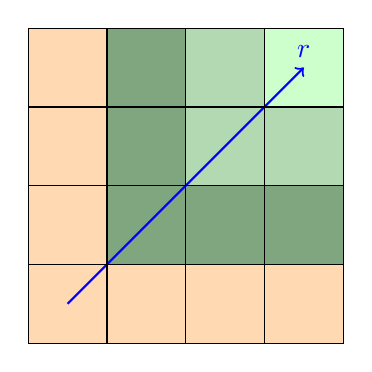
\begin{tikzpicture}[scale=0.5]
	
	\draw[fill=orange!30] (0,0) rectangle +(8,2);
	\draw[fill=orange!30] (0,2) rectangle +(2,6);

	\draw[fill=green!30!black!50] (2,2) rectangle +(6,2);
	\draw[fill=green!30!black!50] (2,4) rectangle +(2,4);
	
	\draw[fill=green!50!black!30] (4,4) rectangle +(4,2);
	\draw[fill=green!50!black!30] (4,6) rectangle +(2,2);
	
	\draw[fill=green!20] (6,6) rectangle +(2,2);
	
	% arrows ...
	\draw[blue, thick, ->] (1,1) -- (7,7) node[above] {$r$}; 
												
	% the grid ...
	\draw[step=2cm] (0,0) grid (8,8);	
	
\end{tikzpicture}
\caption{\small The outermost layer is shown in orange, for which the local expansions are computed directly. The other layers (in green) are computed by propagation. The direction of propagation ($r$) is shown using the arrow and by the shade of the layers, lighter being later in time. 
}
\label{fig:sweep}
\end{figure}

\begin{figure}
\centering
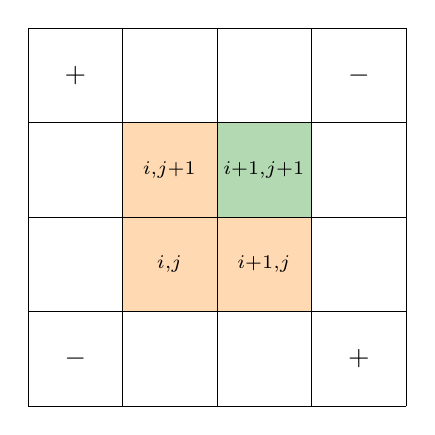
\begin{tikzpicture}[scale=0.6]
	
	\draw[fill=orange!30] (2,2) rectangle +(4,2);
	\draw[fill=orange!30] (2,2) rectangle +(2,4);
	
	\draw[fill=green!50!black!30] (4,4) rectangle +(2,2);		
	% the grid ...
	\draw[step=2cm] (0,0) grid (8,8);	
	
  \draw (3,3) node {$_{i, j}$};
  \draw (5,3) node {$_{i+1, j}$};
  \draw (3,5) node {$_{i, j+1}$};
  \draw (5,5) node { $_{i+1, j+1}$};
	
	\draw (1,1) node {$-$};
	\draw (7,7) node {$-$};
	\draw (1,7) node {$+$};
	\draw (7,1) node {$+$};
			
\end{tikzpicture}
\caption{\small Illustration of the modified sweeping. The local expansions of the boxes shown in orange color are used for computing the local expansion at the box shown in green color. The stencil is given in equation (\ref{eqn:sweep}). Assuming $K = 3$, a simple inspection of the interaction lists reveal that the contributions of boxes marked by ``+'' must be added and those marked by ``-'' must be substracted. }
\label{fig:w2l}
\end{figure}

\subsection{Modified sweeping algorithm for surface distributions} 
\label{sec:mst}
For surface distributions, the algorithm introduced in the previous section suffers from the same problem as the sweeping algorithm in that it generates large number of additional non-empty boxes and consequently it becomes computationally more expensive than the direct scheme. We introduce a new approach here that does not generate any extra non-empty boxes and performs better than the direct scheme. 

The main idea, however, is similar: once a local expansion is formed at a particular box, we use this information to minimize the translation cost at a subsequently visited box. At the first box $B_1$ we form the local expansion directly with $\displaystyle \mathcal{O}\left(\,|\mathcal{I} [B_1]| \, p^3\right)$ work, where $|\cdot|$ is the size of the set. For subsequent boxes, we only need to add/subtract the plane-wave expansions of the boxes that are not present in both the interaction lists of the current box and that of the previously visited box. The problem is therefore to determine the optimal traversal such that the overall cost is reduced.

\begin{prob}[Optimal Traversal] {\em Find an ordering $\{ B_1, B_2, \ldots, B_{|B|}\}$ so that 
%
\beq |\mathcal{I}[B_1]| + \sum_{j=1}^{|B|-1} |\mathcal{I}(B_j)\cup\mathcal{I}(B_{j+1}) \setminus \mathcal{I}(B_j)\cap\mathcal{I}(B_{j+1})| \label{eqn:OT}\eeq
%
is minimized.}
\end{prob}

The first term in equation (\ref{eqn:OT}) is the translation cost of the first box and the term inside the summation encodes the cost of translating the local expansion from $B_j$ to $B_{j+1}$. Note that cost of translating plane-waves between two consequent boxes in the ordering is minimal if their interaction lists have many common elements. There are many ways to find the optimal traversal path. We take a graph theoretic approach by reducing optimal traversal problem to one of finding the minimum spanning tree of a weighted graph. 

\begin{prob}[MST] 
\label{prob:mst}
{\em Construct a weighted graph $G = (V, E)$ with the non-empty FGT boxes as its vertices. 
An edge is introduced between vertices $v_i$ and $v_j$ if and only if $B_i \in \mathcal{I}[B_j]$. The weight of an edge between boxes $B_i$ and $B_j$ is given by
%
\beq w_{ij} = |\mathcal{I}(B_i)\cup\mathcal{I}(B_{j}) \setminus \mathcal{I}(B_j)\cap\mathcal{I}(B_{j})|. \eeq
%
Introduce an additional vertex $v*$ which connects to every vertex $v_i$ in the graph by an edge whose weight is equal to $|\mathcal{I}[B_i]|$. Find the minimum spanning tree of $G$.}
\end{prob}

The vertex $v*$ encodes the cost of the direct computation at the boxes. We compute the minimum spanning tree of this graph using Kruskal's algorithm \cite{kruskal56} whose complexity is $\mathcal{O}(|E| \log |V|)$, which in our case becomes $\mathcal{O}(K^2 |B| \log |B|)$ because $|E| = K^2 |B|$ and $|V| = |B|$. From a practical perspective, it is sufficient to add the edges for the immediate neighbors of a vertex $v_i$, resulting in $|E| = 13 |B|$ in 3D.\footnote{This can result in an increased cost due to direct computation for isolated boxes.} This approach brings down the complexity of determining the optimal path to $\mathcal{O}(|B| \log |B|)$. 

The traversal is then defined by the tree rooted at $v*$. Depending on how the data is stored, the tree can be traversed in a depth-first or a breadth-first fashion. In our implementation, we use a breadth-first traversal. Once the optimal ordering is computed by solving the Problem \ref{prob:mst}, the traslation step is carried out by traversing the tree and forming the local expansion at the box $B_{j+1}$ using the local expansion at $B_j$ and by substracting the contributions of boxes in \[\mathcal{I}[B_j] \setminus \mathcal{I}(B_j)\cap\mathcal{I}(B_{j+1}) \]
and adding the contributions of boxes in 
\[ \mathcal{I}[B_{j+1}] \setminus \mathcal{I}(B_j)\cap\mathcal{I}(B_{j+1}).\] 
The average time complexity of this scheme is $\bigO(K p^3 |B|)$. 
We demonstrate the speed-ups achieved for non-empty box distributions on a sphere in Table \ref{tab:ratio}, Figures \ref{fig:speedup} and \ref{fig:sphere}.
   
%Each of the remaining vertices (FGT boxes) are connected to a maximum of $26$ other vertices (corresponding to the immediate non-zero neighbors of the box). 

{\em A priori cost estimation.} For a given non-empty box distribution, we can estimate the cost of the propogation algorithm  described in Section \ref{sec:sweep} by visiting each non-empty box and counting the number of empty boxes in its interaction list. The worst case complexity of this estimation algorithm is $\bigO(K^3 |B|)$. The operation count for the W2L step via propogation algorithm is $15 p^3 |B_{\text{total}}|$ where $|B_{\text{total}}|$ is the number of non-empty boxes plus the number of empty boxes in their interaction lists. 

The operation count for the W2L step via MST algorithm is $p^3 \mathcal{C}$ where $\mathcal{C}$ is given by (\ref{eqn:OT}). This can be estimated by solving Problem \ref{prob:mst}. Therefore, with a worst case complexity of $\displaystyle \bigO \left((K^3 + \log |B|) |B|\right)$, we can precisely estimate the operation counts for both the algorithms and chose the one with the lowest cost. 

\begin{table}
\caption{The reduction in the complexity of computing the plane-wave translations by using optimal traversal compared to direct computations. Results are presented for $K=9$ and $K=13$. It can be seen that the speedup is proportional to $K$ and scales with $|B|$.}
\centering
\begin{tabular}{cccc} \hline
        $|B|$  &  direct & MST & ratio \\ \hline       
        \multicolumn{4}{c}{}  \\
        \multicolumn{4}{c}{ {\small $K =  9 \quad (\epsilon = 10^{-6})$}}  \\
        \multicolumn{4}{c}{}  \\
         1K & 114K & 18K & 6.3 \\  
        10K & 1M & 182K & 5.88 \\  
       100K & 9.65M & 1.7M & 5.68 \\  
       1M & 96.8M & 17.1M & 5.68 \\  
       \multicolumn{4}{c}{}  \\
       \multicolumn{4}{c}{ {\small $K =  13 \quad (\epsilon = 10^{-12})$}}  \\
       \multicolumn{4}{c}{}  \\
             1K & 238K & 24K & 9.65 \\  
        10K & 2.24M & 264K & 8.48 \\  
        100K & 20.16M & 2.46M & 8.18 \\  
       1M &   200.56M & 24.5M & 8.18 \\   
\hline
\end{tabular} \label{tab:ratio}
\end{table}

\begin{figure}
  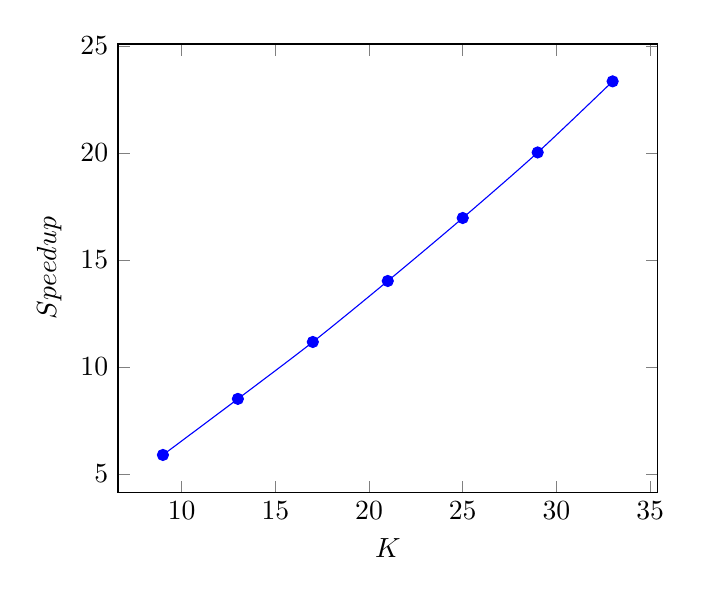
\begin{tikzpicture}
    \begin{axis}[
      xlabel=$K$,
      ylabel=$Speedup$]
      \addplot[smooth,mark=*,blue] plot coordinates {
      (9, 5.88)
      (13, 8.5)
      (17, 11.16)
      (21, 14.01)
      (25, 16.9535)
      (29, 20.0165)
      (33, 23.3387)
      };
      % \addlegendentry{Direct}

    \end{axis}
  \end{tikzpicture}
  \caption{Speedup obtained for increasing values of the size of the interaction list, $K$, for a fixed geometry. The speedup is proportional to $K$ and the complexity of computing the translations is reduced from $\mathcal{O}(K^2|B|)$ to $\mathcal{O}(K|B|)$.}  \label{fig:speedup}
\end{figure}  
%
\begin{figure}
\centering 	

\begin{tikzpicture}
\begin{axis}[
	view={120}{40},
width=220pt,
height=220pt,
grid=major,
z buffer=sort,
xmin=3,xmax=25,
ymin=3,ymax=25,
zmin=3,zmax=25,
enlargelimits=upper,
%xtick={1,11,...,29},
%ytick={1,11,...,29},
%ztick={1,11,...,29},
xlabel={$X$},
ylabel={$Y$},
zlabel={$Z$},
colorbar,
colormap={summap}{
color=(blue);
color=(violet);
%color=(orange); 
color=(red)
},
scatter/use mapped color={
draw=mapped color,fill=mapped color!70},
]
\addplot3[only marks,scatter,mark=cube*,mark size=4,point meta={\thisrow{col}}]
table[x=xc,y=yc,z=zc]{sphere_mst.dat};
\end{axis}
\end{tikzpicture}

% 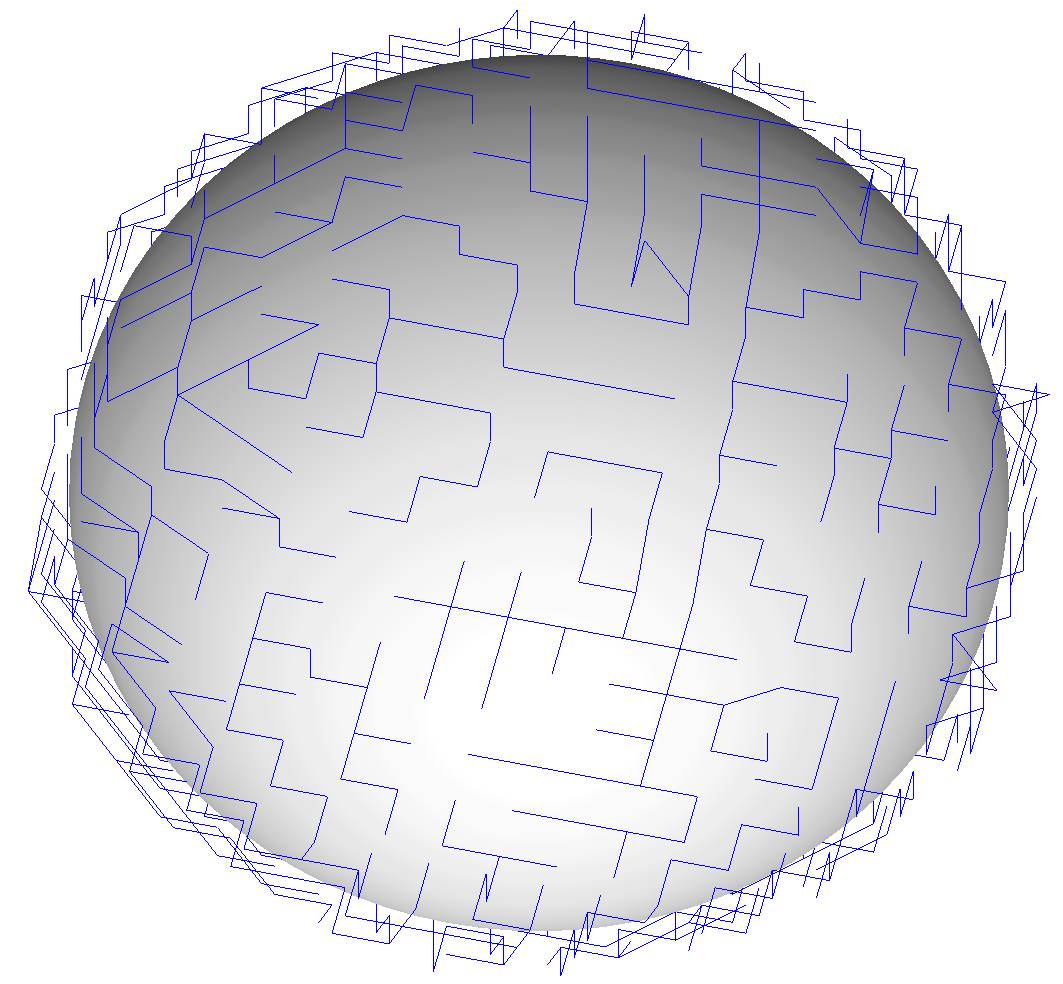
\includegraphics[width=0.4\textwidth]{figs/sphere_mst}
\caption{The cost of translations for the optimal traversal path for a spherical shell distribution ($K=9$). The boxes $B_i$ are color coded based on the cost of performing the translation. For comparison the average cost for direct translations in this case is $99$.} \label{fig:sphere}
\end{figure}

